%!TEX root = ../dissertation.tex
% this file is called up by thesis.tex
% content in this file will be fed into the main document

\graphicspath{{8-conclusions/figures/}}

\chapter{Conclusions and Final Remarks}
\label{ch:conclusions}

This thesis have presented a number of novel approaches showing the effectiveness of employing deep generative models in automatic music transcription research.
In this chapter, we summarize the findings and provide the future prospects in this line of research.

\section{Summary and Takeaways}

\TODO{Answer the questions}

\begin{enumerate}
	\item What kinds of deep models and representations can be used for effectively extracting pitch from audio?
	\item How does the choice of datasets affect the accuracy and the generalizability of a trained model?
	\item How can we encode the concept of timbre in a way that is useful for music synthesis and transcription?
	\item How can a transcription model make informed predictions incorporating the knowledge of music theory?
	\item Can a music synthesizer component based on a deep generative model be used to improve music transcription?
\end{enumerate}

\begin{itemize}
	\item Dataset matters (highly correlated than images ~\cite{thickstun2018invariances})
	\item Prior knowledge matters in all domains
\end{itemize}


\section{Future Research Directions}

In this section, we discuss how the automatic music transcription approaches discussed in this thesis can be extended and further improved in future research.
An immediate future research direction is to combine the findings of Chapter~\ref{ch:adversarial} and Chapter~\ref{ch:timbre} to create a music transcription system with both an adversarial discriminator and an appended synthesizer component.
Although left as out-of-scope in this thesis because of the computational constraints, this will in theory provide better regularization for the overall system and be able to achieve better performance in music transcription.

Data augmentation can provide additional improvement in most music analysis tasks~\cite{mcfee2015muda}, although it was not considered in the experiments in this thesis, in order to keep the narratives focused on the novel approaches being introduced in each chapter.
While the conventional methods such as time stretch and pitch shift can be used for the purpose of music data augmentation, expressive music language models and music synthesis models can provide more powerful means of enriching the distribution of music data for training a transcription model.
This idea is illustrated in Figure~\ref{fig:unlimited-data}; an unlimited source of training data can be created using a combination of a powerful music language model and a good music synthesizer.
This idea is particularly promising considering the incredible performance of the recent transformer-based language models, 
\TODO{cite Transformer (Attention is all you need), GPT}, which have been shown to be also effective in producing coherent symbolic music \cite{huang2019transformer}.

More powerful computational hardware in the future will enable a longer context length to be used in larger transformer models, which suggests another intriguing future research direction to learn a music language model in the audio waveform domain.
This will help create a more expressive synthesizer component, which can be used to augmenting a music transcription model.
A compression method such as VQ-VAE~\cite{oord2017vqvae} would be helpful in allowing even longer context length to be used in such language model.


\begin{figure}
\centering
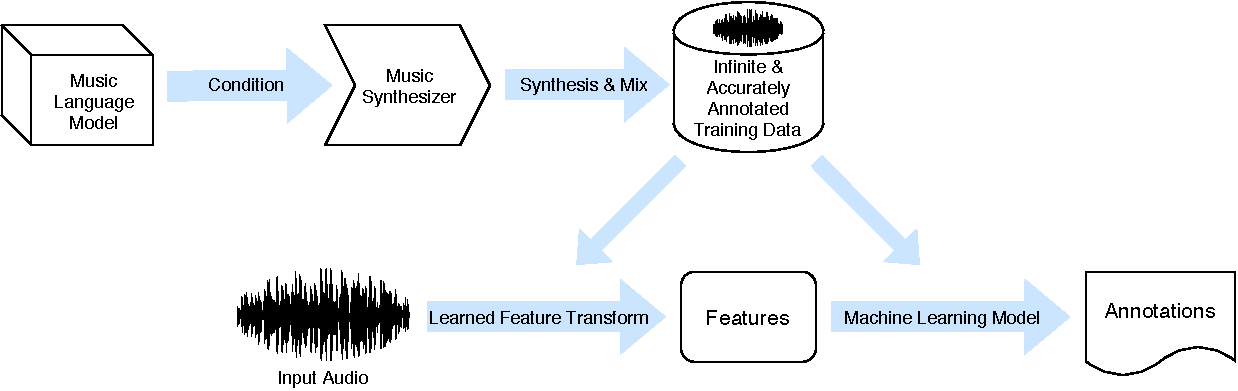
\includegraphics[width=\textwidth]{paradigms-5-proposed.pdf}
\caption{A combination of music language model and music synthesizer can be used as an infinite source of accurately annotated training data for a transcription model.}\label{fig:unlimited-data}
\end{figure}


Finally, in the discussion regarding the future of AMT, we need to consider the fundamental limitation on any music transcription task, either automatic or manual, and when it can be said that AMT is solved.
Polyphonic music contains a mixture of sounds with an indefinite number of notes being played simultaneously; even the most experienced musicians may not be able to identify every note, and the audio mixture may not contain the sufficient information to convey all notes in the first place.
It would be unreasonable to expect anyone to perfectly transcribe all notes in the score of an orchestral music from an audio file, but it would be sensible for a trained musician to produce a version of score that, when played by the same orchestra, sounds indistinguishable to the original recording.
Considering these limitations, passing this ``transcriptional Turing test'' as shown in Figure \ref{fig:turing}, rather than achieving the 100\% accuracy on a certain dataset, should be the ultimate goal of automatic music transcription, at which point it can be said to have a human-level intelligence on this task.

\begin{figure}
	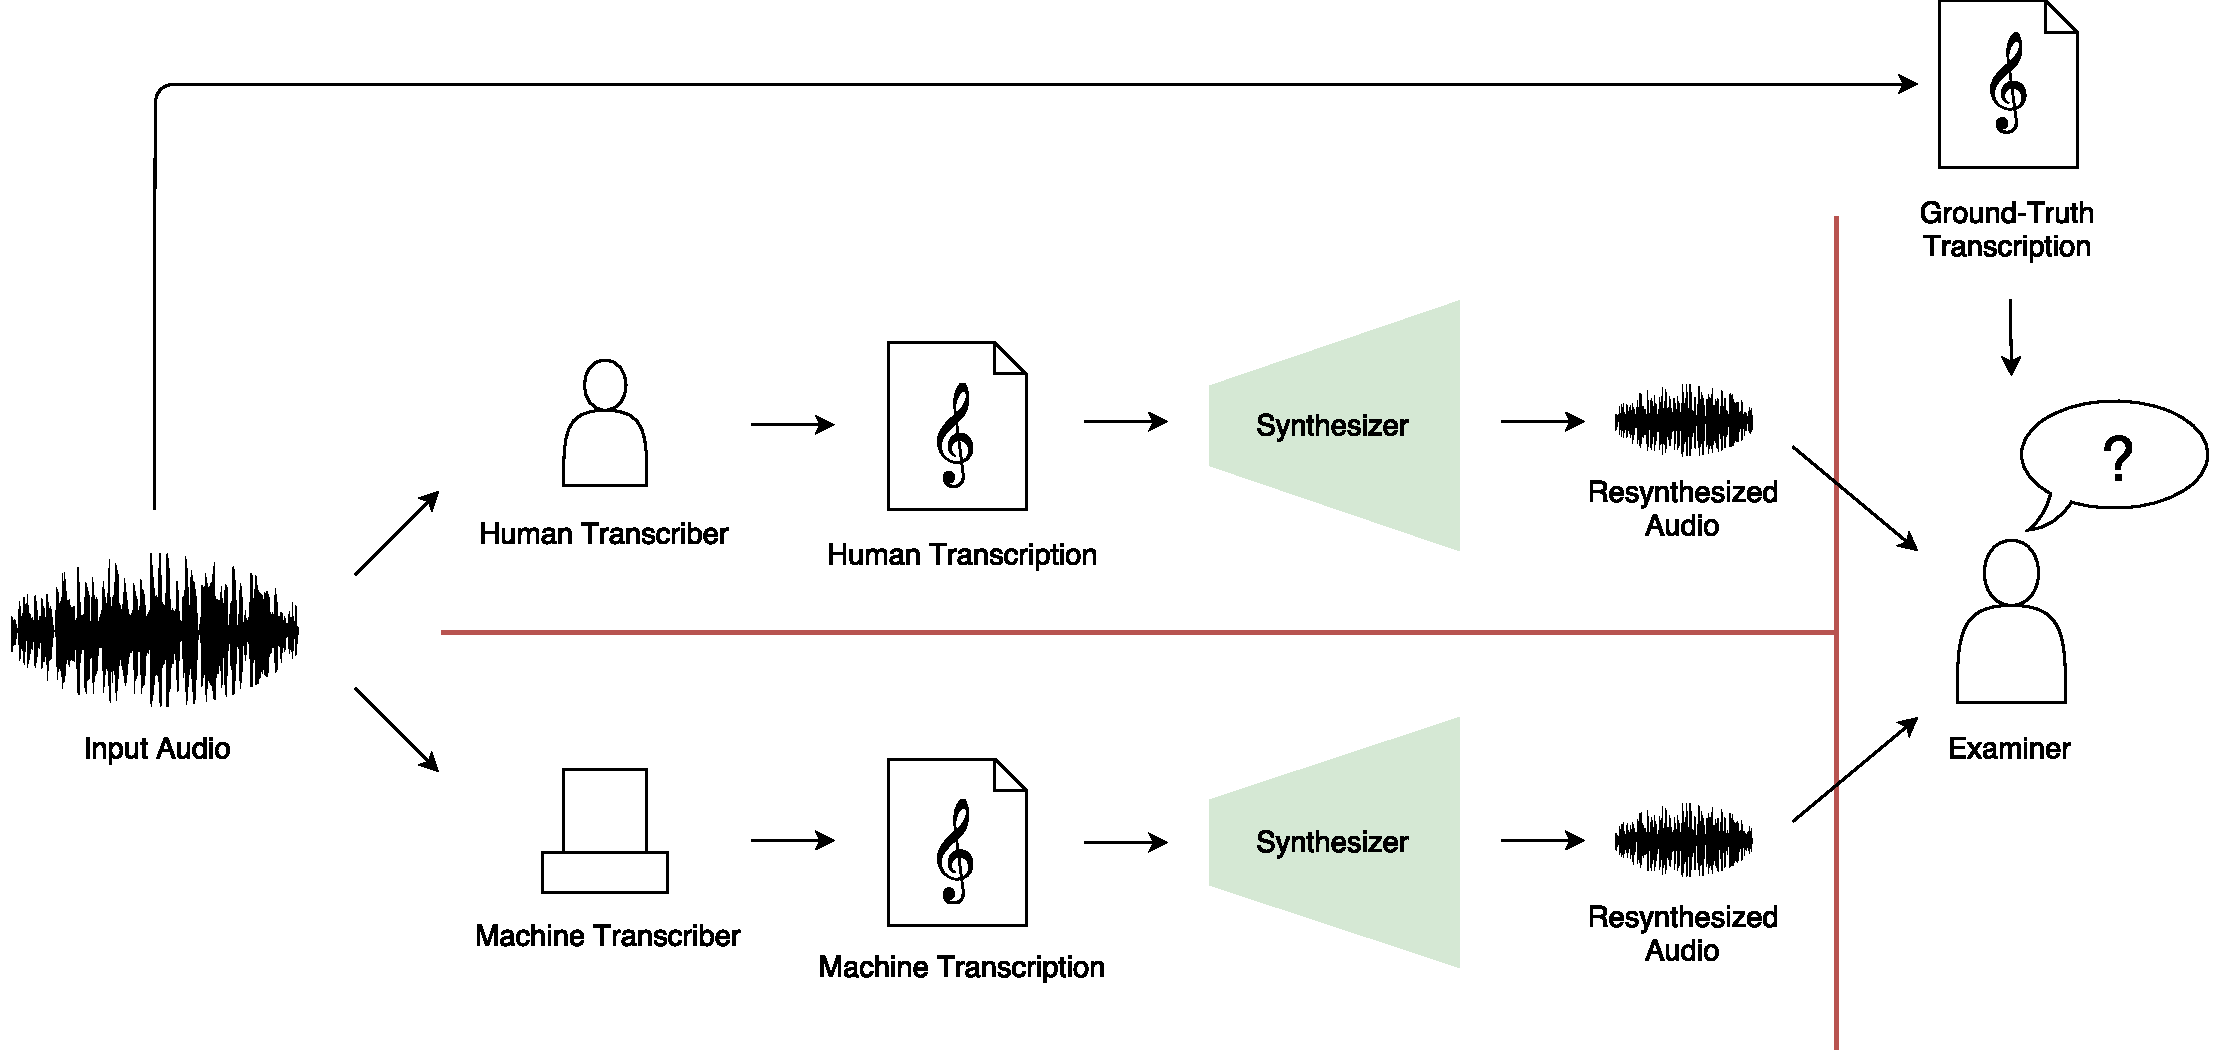
\includegraphics[width=\textwidth]{turing.pdf}
	\caption{The \emph{transcriptional Turing test}, to test whether an automatic music transcription algorithm has reached human-level. While this provides some conceptual insights to the adversarial training setup, to be covered in the later chapters, fully achieving the human-level performance is out of scope of this thesis.}
	\label{fig:turing}
\end{figure}

\TODO{finish with a bright future prospect}

\pagebreak